\section{Consultar Información de Tratamientos}

Un paciente podrá consultar la información de un tratamiento que se encuentre en estado activo, en donde se mostrará el doctor que lo expidió, la fecha en que se expidió, el estado y una vista de las semanas en que ese tratamiento ha estado en función.

\subsubsection{Procedimiento}
\begin{enumerate}
	
	\item Selecciona un tratamiento en estado activo de la pantalla \textbf{Tratamientos}.

	\begin{figure}[!htbp]			
		\hypertarget{fig:Tratamientos2}{\hspace{1pt}}
		\begin{center}
			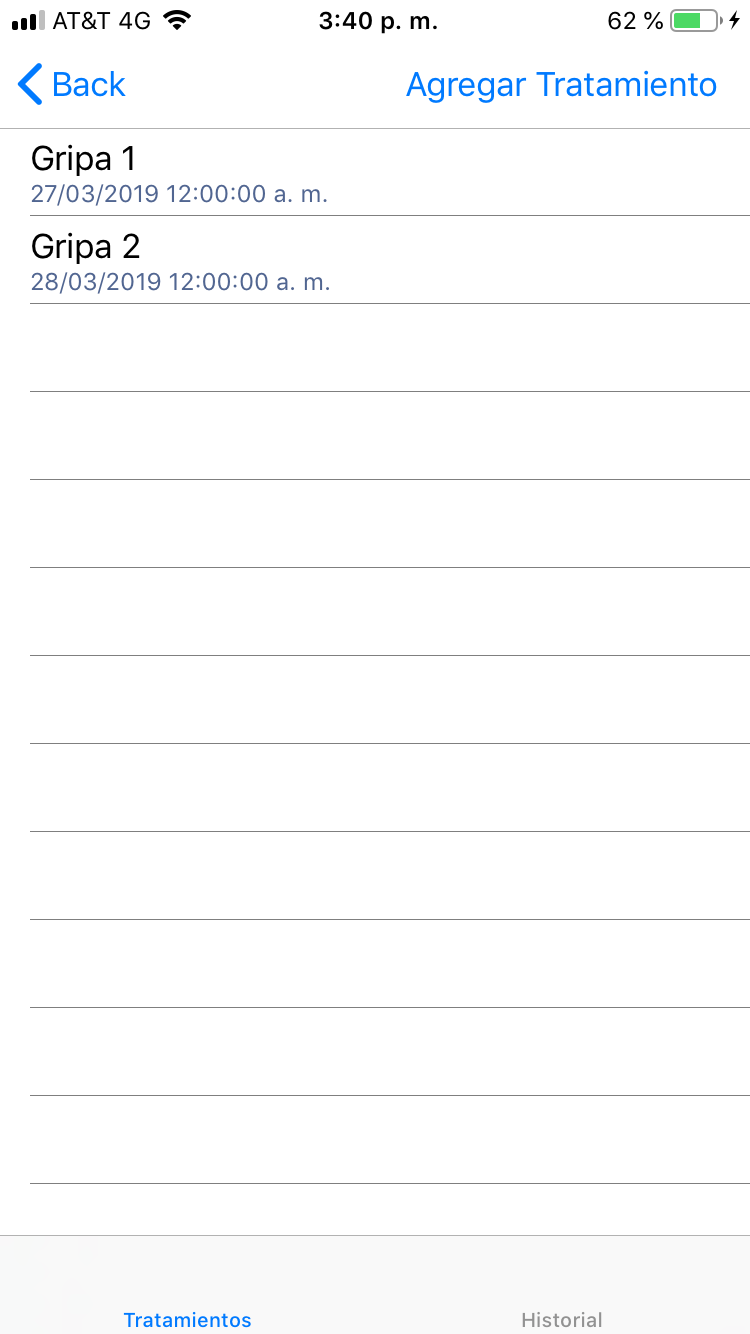
\includegraphics[height=0.4\textheight]{Paciente/InfoTratamiento/images/Tratamientos}
			\caption{Tratamientos}
			\label{fig:Tratamientos2}
		\end{center}
	\end{figure}

	\item Se mostrará la pantalla \textbf{Información de Tratamiento}. 
	\newpage
	
	\begin{figure}[!htbp]			
		\hypertarget{fig:infoTratamiento}{\hspace{1pt}}
		\begin{center}
			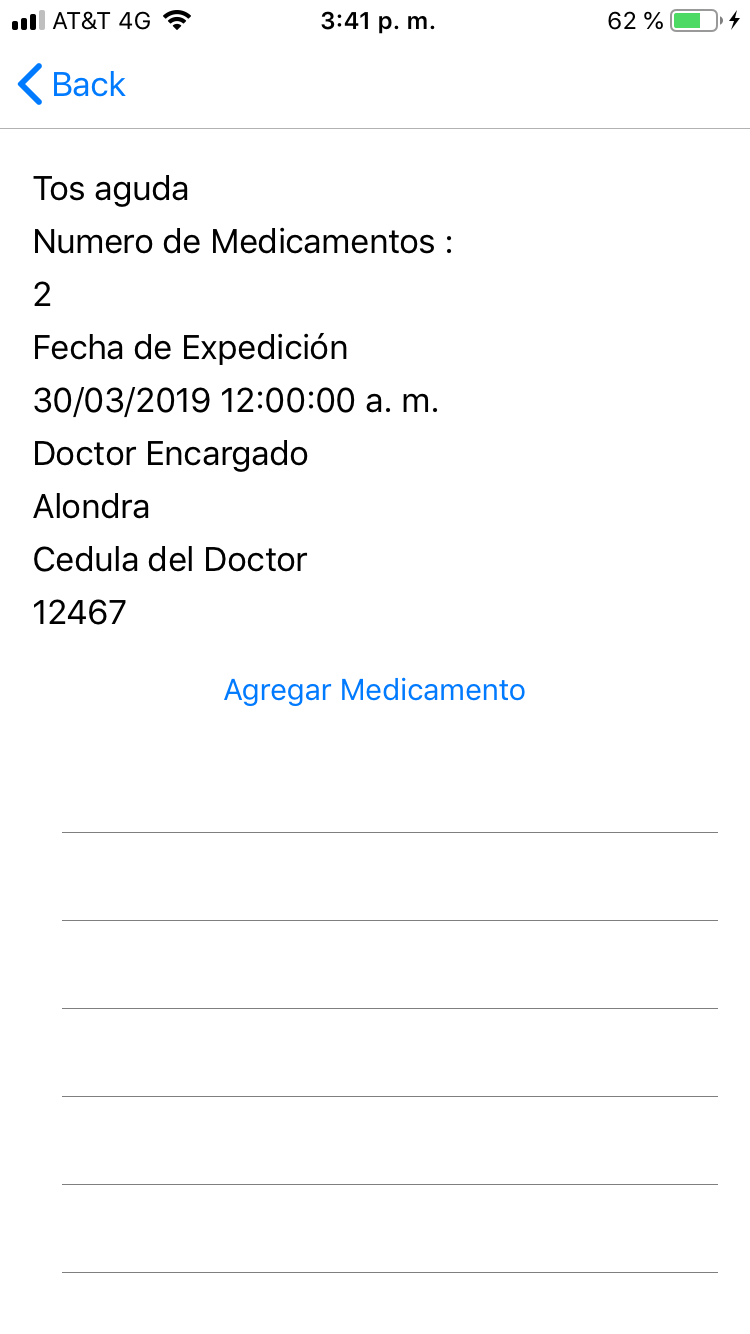
\includegraphics[height=0.4\textheight]{Paciente/InfoTratamiento/images/infoTratamiento}
			\caption{Información de Tratamiento}
			\label{fig:infoTratamiento}
		\end{center}
	\end{figure}
	
\end{enumerate}

